%-----------------------------------LICENSE------------------------------------%
%   This file is part of tikz_figures.                                         %
%                                                                              %
%   tikz_figures is free software: you can redistribute it and/or              %
%   modify it it under the terms of the GNU General Public License as          %
%   published by the Free Software Foundation, either version 3 of the         %
%   License, or (at your option) any later version.                            %
%                                                                              %
%   tikz_figures is distributed in the hope that it will be useful,            %
%   but WITHOUT ANY WARRANTY; without even the implied warranty of             %
%   MERCHANTABILITY or FITNESS FOR A PARTICULAR PURPOSE.  See the              %
%   GNU General Public License for more details.                               %
%                                                                              %
%   You should have received a copy of the GNU General Public License along    %
%   with tikz_figures.  If not, see <https://www.gnu.org/licenses/>.           %
%------------------------------------------------------------------------------%

% Use the standalone class for displaying the tikz image on a small PDF.
\documentclass[crop, tikz]{standalone}

% Import the tikz package to use for the drawing.
\usepackage{tikz}

% Needed for \mathbb command.
\usepackage{amssymb}

% Begin the document.
\begin{document}

    % Draw the figure.
    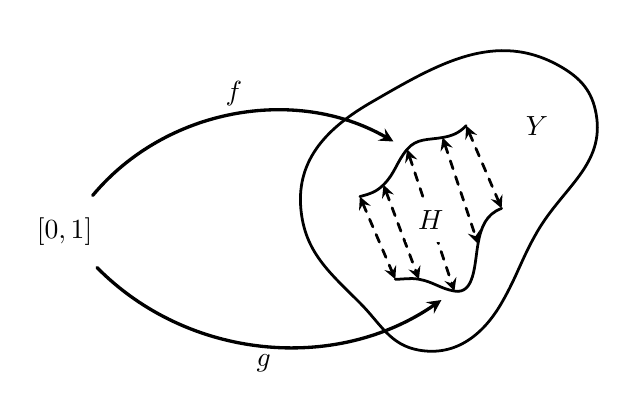
\begin{tikzpicture}[%
        line width = 1pt,
        line cap = round,
        scale = 1.5,
        > = stealth,
        every edge/.style = {%
            draw = black,
            very thick
        },
        smalldot/.style = {
            circle,
            fill = black,
            inner sep = 0,
            outer sep = 0
        },
        dashcurve/.style = {
            draw = black,
            dashed,
            <->
        }
    ]

        % Set points for upper curve.
        \coordinate (a0) at (2.5, 1.3);
        \coordinate (b0) at (2.7, 1.4);
        \coordinate (c0) at (2.9, 1.7);
        \coordinate (d0) at (3.2, 1.8);
        \coordinate (e0) at (3.4, 1.9);

        % Set points for lower curve.
        \coordinate (a1) at (2.8, 0.6);
        \coordinate (b1) at (3.0, 0.6);
        \coordinate (c1) at (3.3, 0.5);
        \coordinate (d1) at (3.5, 0.9);
        \coordinate (e1) at (3.7, 1.2);

        % Points for the outer blob.
        \coordinate (a2) at (3.0, 0.0);
        \coordinate (b2) at (2.5, 0.4);
        \coordinate (c2) at (2.0, 1.2);
        \coordinate (d2) at (2.6, 2.1);
        \coordinate (e2) at (4.2, 2.4);
        \coordinate (f2) at (4.5, 2.0);
        \coordinate (g2) at (4.0, 1.0);
        \coordinate (h2) at (3.7, 0.4);

        % Nodes labelling the domain and co-domain.
        \node at (0.0, 1.0) (I) {$[0,1]$};
        \node at (4.0, 1.9) {$Y$};

        % Draw upper curve.
        \draw (a0) to [out = 15, in = -135]
              (b0) to [out = 45, in = -130]
              (c0) to [out = 50, in = -170]
              (d0) to [out = 10, in = -135] (e0);

        % Draw lower curve.
        \draw (a1) to [out = 0, in = 170]
              (b1) to [out = -10, in = 170]
              (c1) to [out = -10, in = -100]
              (d1) to [out = 80, in = -160] (e1);

        % Draw dashed lines connecting curves.
        \begin{scope}[<->, dashed]
            \draw (a0) to (a1);
            \draw (b0) to (b1);
            \draw (c0) to node[inner sep = 1ex, fill = white] {$H$} (c1);
            \draw (d0) to (d1);
            \draw (e0) to (e1);
        \end{scope}

        % Draw curve defining the blob.
        \draw (a2) to [out = 170, in = -45]
              (b2) to [out = 135, in = -85]
              (c2) to [out = 95, in = -150]
              (d2) to [out = 30, in = 150]
              (e2) to [out = -30, in = 100]
              (f2) to [out = -80, in = 60]
              (g2) to [out = -120, in = 60]
              (h2) to [out = -120, in = -10] cycle;

        % Draw curves representing maps f and g.
        \begin{scope}[%
            shorten > = 0.2cm,
            shorten < = 0.2cm,
            ->
        ]
            \path (I) edge[bend left = 40] node[above] {$f$} (c0);
            \path (I) edge[bend right = 40] node[below] {$g$} (c1);
        \end{scope}
    \end{tikzpicture}
\end{document}
